\chapter{Implementation} \label{appendix:implementation}

This appendix explains how the current dynamic action discovery is implemented in ASP.NET Core. It then covers the parts that must be removed to disable the dynamic action discovery. Finally, it covers how the static action discovery is implemented using source generators, the output of such a source generator, and how it can be used to improve application startup speed.

\section{Current Implementation of Dynamic Action Discovery in ASP.NET Core}

Web applications primarily respond to user requests, and while hardcoding each endpoint and its response would theoretically serve this purpose, it's not a practical solution when dealing with hundreds of endpoints. ASP.NET Core handles this challenge by using controllers—classes that group related actions and automate endpoint mapping through attributes. Figure \ref{fig:controller} illustrates an example of such a controller.

\begin{figure}[H]
\centering
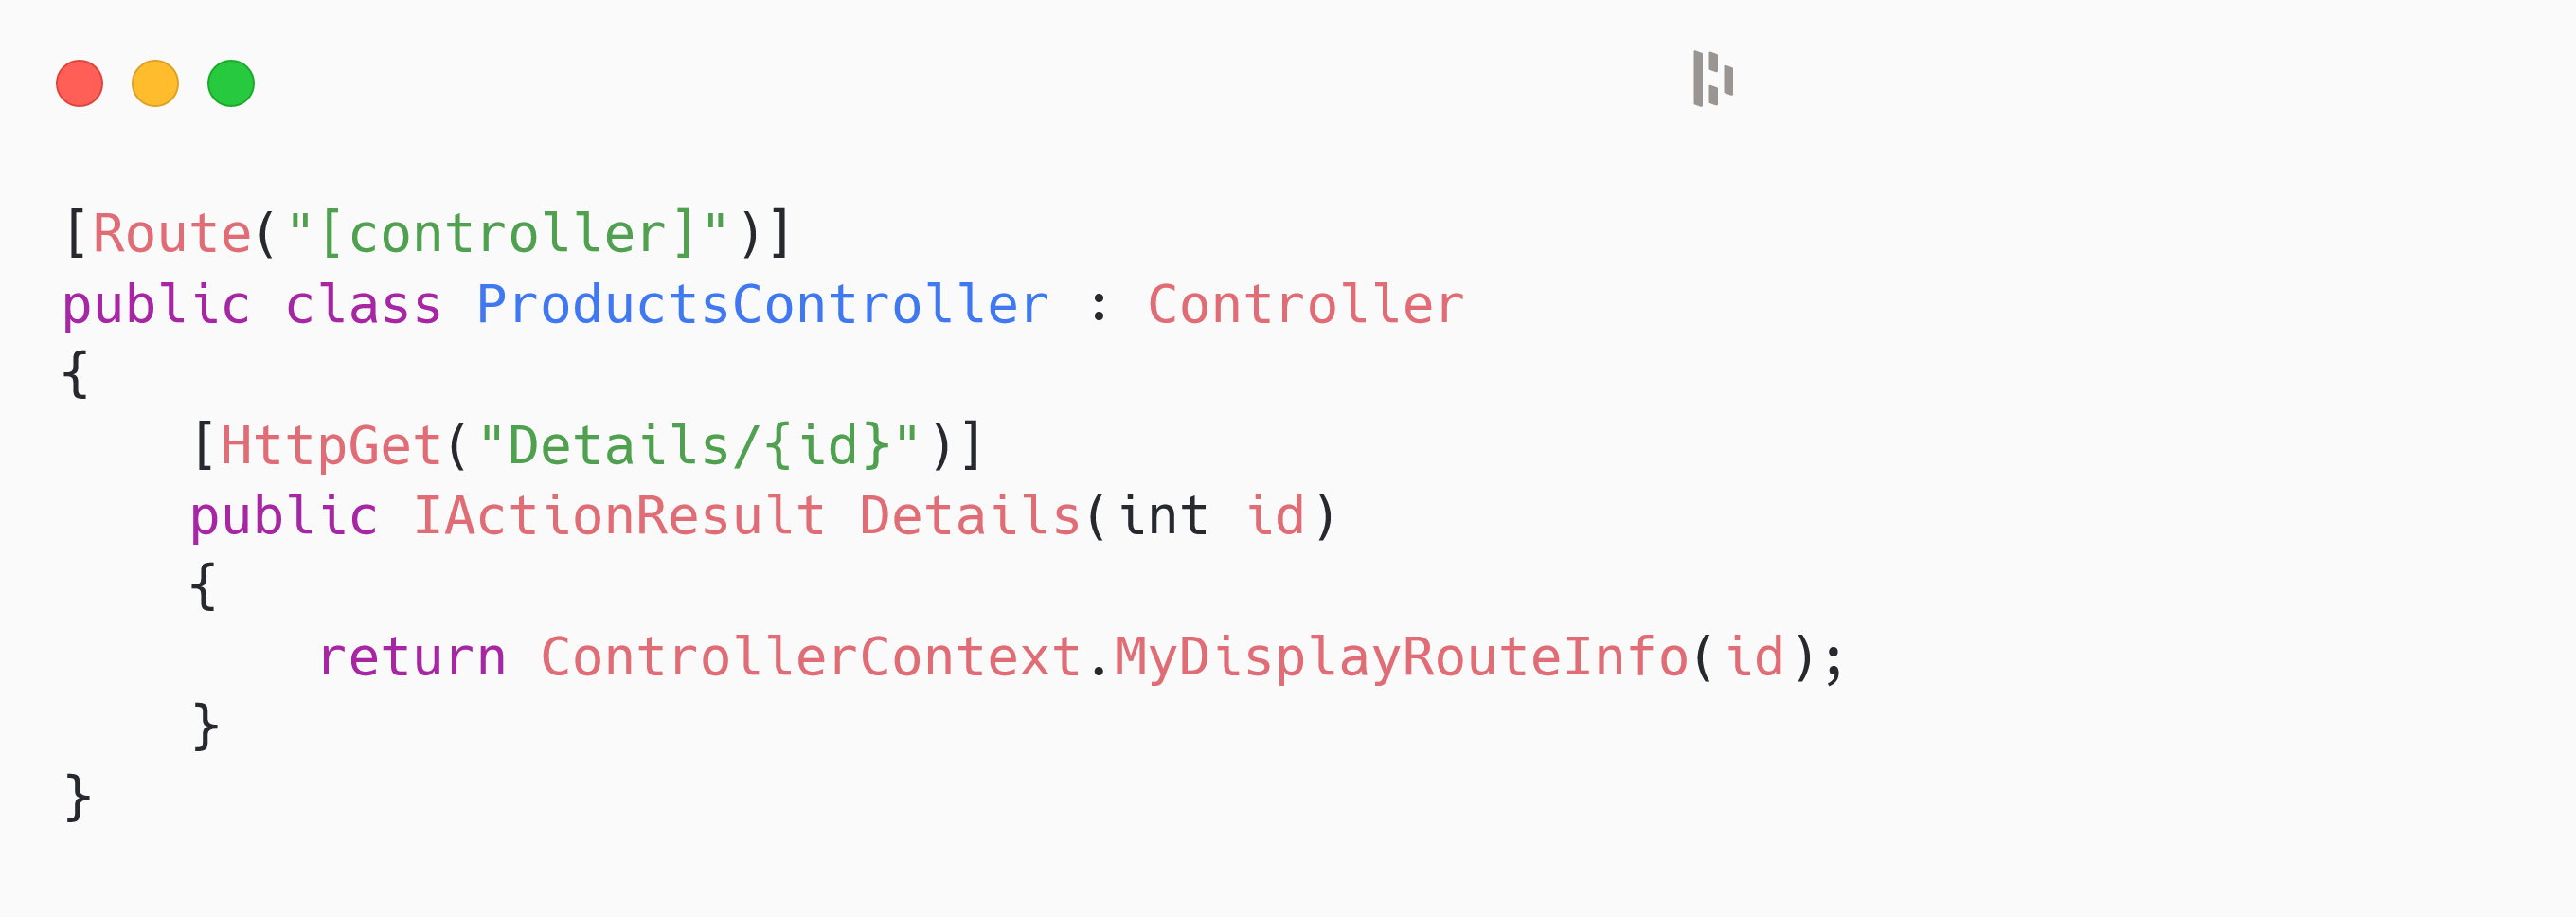
\includegraphics[width=1\textwidth]{graphics/attribute-routing.png}
\caption{An example controller using attributes in ASP.NET Core}
\label{fig:controller}
\end{figure}

In ASP.NET Core, endpoint mapping automation, also known as "action discovery," is achieved by dynamically scanning the entire codebase during the application's startup phase. However, this dynamic action discovery relies on specific services and middleware incorporated into the application at different stages of the startup phase. Figure \ref{fig:startup-phase} shows the startup phase of an ASP.NET Core application and the order of adding services and middleware.

\begin{figure}[H]
\centering
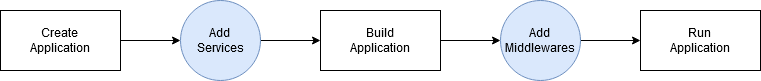
\includegraphics[width=1\textwidth]{graphics/startup-phase.png}
\caption{Flow of the application startup process in ASP.NET Core}
\label{fig:startup-phase}
\end{figure}

ASP.NET Core follows a specific sequence during application setup:

\begin{enumerate}
    \item An application is created, and required services are added to the Dependency Injection (DI) container. Classes can then define their dependencies in their constructor, and the DI container automatically resolves these dependencies to the correct implementation.
    \item The application is built, incorporating the registered services.
    \item Middlewares are added. These components can influence how an ASP.NET Core application handles each request.
    \item The application is started.
\end{enumerate}

In this startup sequence, the dynamic action discovery involves a middleware and a mapper before the application starts. The middleware in question is the routing middleware, which relies on the mapper's output to route requests to the correct actions.

The mapper is invoked when using methods like \texttt{MapControllers}, which generate the application model—a representation of all controllers and their actions in the application. The process is visualized in Figure \ref{fig:sequence-diagram} as a sequence diagram.

\begin{figure}[H]
\centering
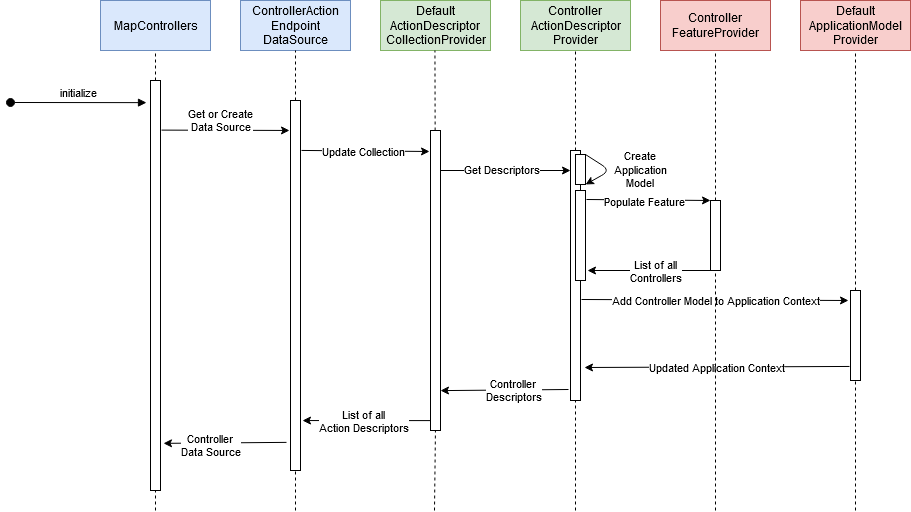
\includegraphics[width=1\textwidth]{graphics/Sequence Diagram.drawio.png}
\caption{Sequence diagram illustrating the application model creation process}
\label{fig:sequence-diagram}
\end{figure}

The sequence of operations leading to action discovery in ASP.NET Core begins when a developer calls the mapping method, such as \texttt{MapControllers}. This method, identified in blue in Figure \ref{fig:sequence-diagram}, initiates the process of endpoint mapping.

Upon invocation, \texttt{MapControllers} creates an instance of the \texttt{ControllerActionEndpointDataSource} (highlighted in blue). This class generates a collection of endpoints, which form the building blocks of the application's routing mechanism. Each endpoint encapsulates essential information, such as the target action (method) to be executed upon a specific user request.

To generate this collection of endpoints, the \texttt{ControllerActionEndpointDataSource} class needs to obtain an overview of all available actions in the application. It requests an \texttt{IActionDescriptorCollectionProvider} from the DI container. Per default, this resolves to the \texttt{DefaultActionDescriptorCollectionProvider}. It then indirectly calls the \texttt{UpdateCollection} method of the \texttt{DefaultActionDescriptorCollectionProvider}. This action description provider fetches all the registered \texttt{ActionDescriptorProvider} services from the DI container and executes them, thereby gathering actions from various sources.

One specific \texttt{ActionDescriptorProvider} service of interest here is the \texttt{ControllerActionDescriptorProvider} (marked in green). This service holds the key to our focus area: the actions within the application's controllers. This service creates an application model that comprehensively represents all controller-related information.

The \texttt{ControllerActionDescriptorProvider} works through three sequential phases:

\begin{enumerate}
    \item \textbf{Creation of an Application Model}: An empty application model is initialized. This model is designed to hold all relevant information about the controllers in the application and their associated actions.

    \item \textbf{Controller Discovery}: The \texttt{ControllerActionDescriptorProvider} calls all available \texttt{FeatureProviders} in the DI container, which by default is only the \texttt{ControllerFeatureProvider} (marked red). The \texttt{ControllerActionDescriptorProvider} then calls the \texttt{PopulateFeature} method of every \texttt{FeatureProvider} to identify all controllers within the application. The \texttt{ControllerFeatureProvider} scans all application parts, which are assemblies that reference the MVC package from ASP.NET Core and could contain controllers. This means that by default, all dependencies that use the MVC package, like Swagger, are analyzed as well. Using reflection, the \texttt{PopulateFeature} method analyzes all classes within these assemblies using reflection, extracting those that qualify as controller classes. These discovered controllers are then added to the application model.

    \item \textbf{Model Population}: The \texttt{ControllerActionDescriptorProvider} proceeds to call all available \texttt{ApplicationModelProviders} in the DI container. These providers populate the application model with detailed information about the actions within each identified controller. The most important \texttt{ApplicationModelProvider} is the \texttt{DefaultApplicationModelProvider} (marked red), which loops over the found controllers and extracts their actions along with any associated attributes. The service then creates 'selectors' for each action that holds information about the action's route, the HTTP method (GET, POST, DELETE, etc.), a unique name for the action, and other relevant metadata.
\end{enumerate}

After these three phases, the \texttt{ControllerActionDescriptorProvider} has effectively created an application model containing all the information about the application's controllers. This model is sent back up the call stack to the \texttt{MapControllers} method, which compiles this information into Endpoint objects. The routing mechanism uses these endpoint objects to route incoming requests to the correct actions appropriately.

The key takeaway is that the services marked in red in Figure \ref{fig:sequence-diagram}—the \texttt{ControllerFeatureProvider}, and \texttt{DefaultApplicationModelProvider}—play crucial roles in dynamic action discovery and need to be replaced for static action discovery. The objects marked in blue represent objects that are either directly called by the developer or instantiated without dependency injection and can not be modified. The green objects represent services that can be modified by changing the implementation in the DI container but do not use reflection and therefore do not need to be modified by the static action discovery. Optimizing the startup performance of the application involves substituting the services marked red with custom implementations of the same interfaces designed to employ static action discovery. The creation of the static action discovery is the focus of the next chapter.

\section{New Implementation}

The process of transforming dynamic action discovery into static action discovery can be divided into two primary parts. The first part involves eliminating the services that trigger dynamic action discovery, and the second part necessitates the generation of an IApplicationModelProvider for every controller in the application, accompanied by a service extension method that registers them all on the DI container.

\subsection{Disabling dynamic action discovery}

The first part is pretty straightforward once the underlying problem has been recognized. ASP.NET Core offers the AddMvcCore method, which introduces over 90 services to the DI container. Most of these services are vital for an MVC application to function correctly. Earlier, we pinpointed the services that trigger the dynamic action discovery. We can modify the AddMvcCore method to introduce an optional parameter that inhibits these services from being added when set to false.

To begin with, we prevent the addition of the ControllerFeatureProvider, which disables the system from scanning the application for controllers. Subsequently, we also stop the DefaultApplicationModelProvider and ApiBehaviourApplicationModelProvider from being added. These services are instances of IApplicationModelProvider and would typically analyze all discovered controllers and append information about the containing actions to the application model.

Modifying the internal AddMvcCore method ensures the services are never registered, eliminating the need to filter through all services to remove them after their addition. This reason primarily drove the decision to modify the official ASP.NET Core app rather than crafting an external NuGet.

\subsection{Generating code for the static action discovery}

The next stage involves establishing a new project that contains the actual source generator (the source code for this can be found \href{https://github.com/jorgeparavicini/aspnetcore/tree/feature/static-mvc/src/Mvc/Mvc.Generators/src}{here} \footnote{\url{https://github.com/jorgeparavicini/aspnetcore/tree/feature/static-mvc/src/Mvc/Mvc.Generators/src}}). When building an incremental source generator, the first step is identifying the syntax nodes required to generate the new source code. Doing so boosts performance during development since it enables us to specify the conditions under which our generator should operate. Only when the syntax of these conditions alter, for instance, when a controller class is modified, will the source generator run. Given that we aim to create an application model based on controllers, we need to gain access to all controllers in the application. Therefore, our condition is any class that qualifies as a valid MVC controller. This condition allows us to access the syntax tree of each controller. However, we also require access to the semantic model to glean information about the meaning of the code we are parsing. Lastly, since we need to add data from all controllers to the application model in one call, we must combine every controller's syntax trees into a single IncrementalValueProvider. After all these steps, we can generate the code for the controllers.

Once all the controllers and their semantic models have been identified, we generate a new class for each controller. This class implements the IApplicationModelProvider interface, which consists of two methods and a property. The Order property determines the execution sequence of all the ApplicationModelProviders. We deliberately assign a value less than zero to ensure they execute before other providers, extracting and adding all controller actions to the application model. This step is crucial as most other ApplicationModelProviders need these actions to extend the application model.

The IApplicationModelProvider interface also has a method, OnProvidersExecuted, which we can ignore for our purposes as it executes after all other providers. Essential for us is the OnProvidersExecuting method, which carries out the static action discovery. Here, we generate a ControllerModel that includes the controller's name, derived from the class name, and its selectors and filters. These filters and selectors permit the routing mechanism to determine if requests can be routed to a particular controller. We repeat a similar step for every action within the controller, but instead of creating a ControllerModel, we generate an ActionModel. These ActionModels describe our application's endpoints.

Our method that creates the ApplicationModel resembles the DefaultApplicationModel, albeit with most of the logic executed within the source generator, not at runtime. This decreases runtime complexity, although it's not always possible. For instance, extracting the HTTP method to create a selector for an ActionModel is tricky. The routing middleware only directs requests to an endpoint if the action explicitly accepts that HTTP method. This prevents unwanted situations, like executing endpoints that delete business resources via a GET query. However, this extraction process isn't deterministically generable because any attribute implementing the IActionHttpMethodProvider can set an action's HTTP method. This interface requires the attributes to define a property that does not have to be a compile-time constant.  Figure \ref{fig:action-provider} shows the generated code by our source generators to overcome this restriction.

\begin{figure}[H]
\centering
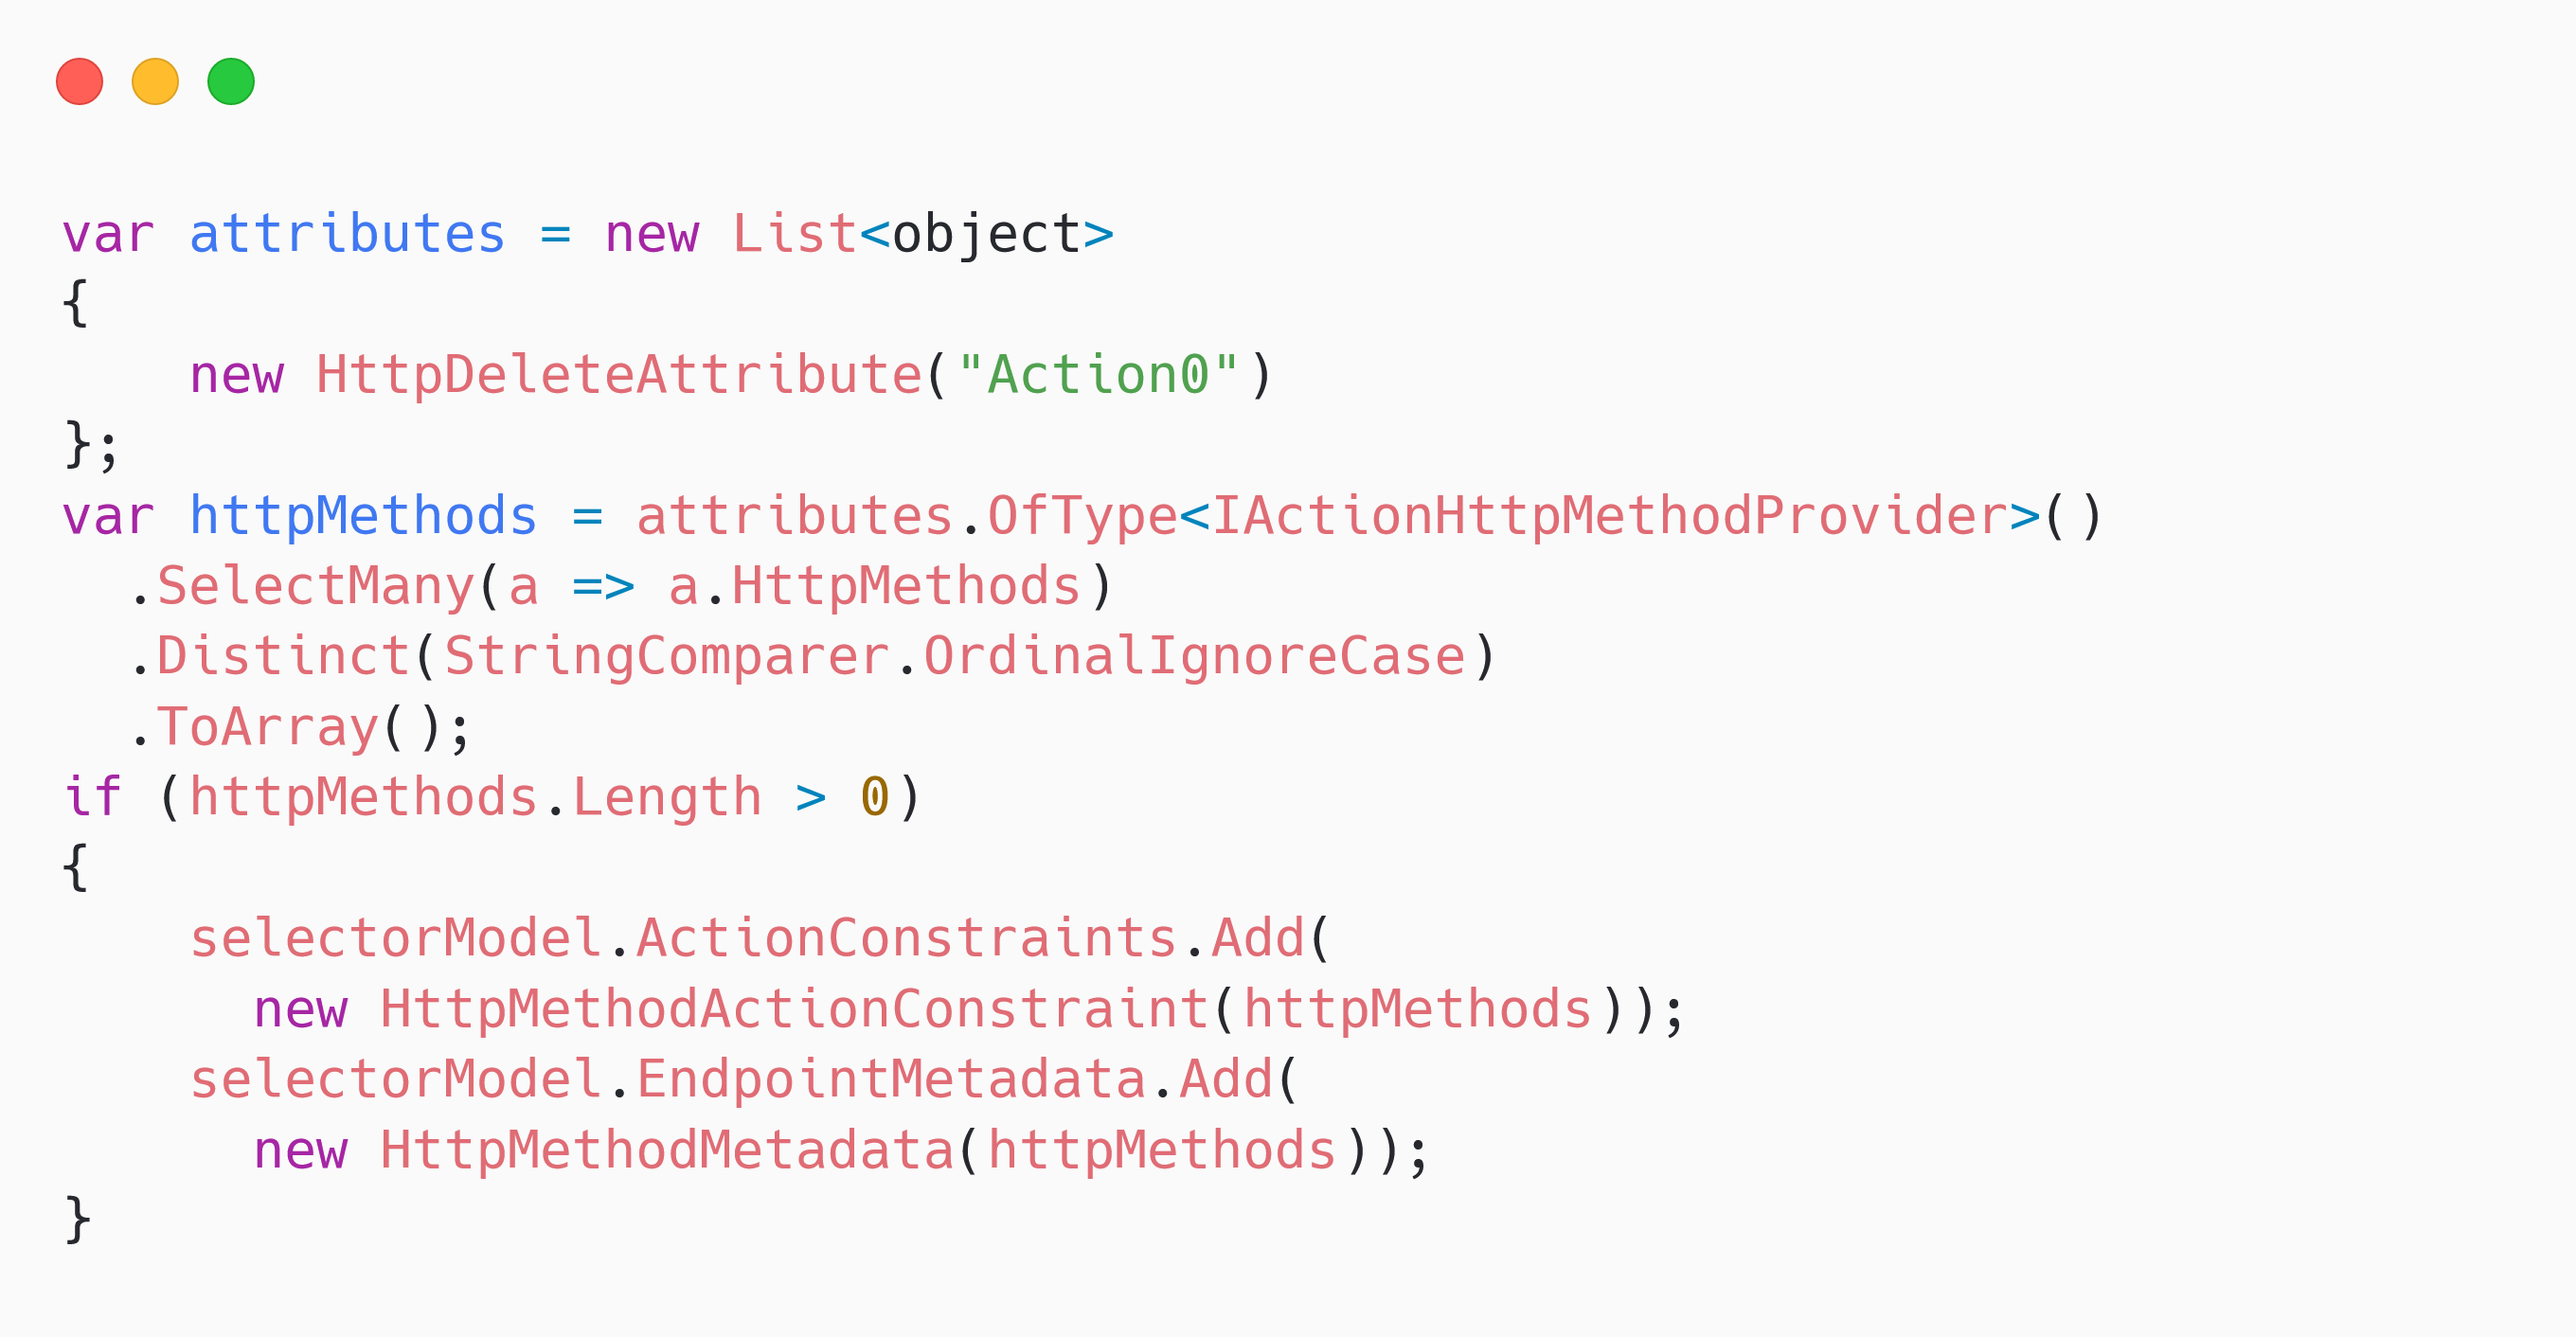
\includegraphics[width=1\textwidth]{graphics/action_http_method_provider.png}
\caption{Extracting and applying HTTP methods from action attributes}
\label{fig:action-provider}
\end{figure}

This code snippet demonstrates how the HTTP methods an action supports are parsed. All its attributes are instantiated first; then, the HTTP methods are extracted from them. The parsed methods are then assigned to the endpoint metadata and action constraints that define the action. It should be essential to note that the attributes must be instantiated the same way as they are declared in the source code because the parameters may influence the \texttt{IActionHttpMethodProvider}s \texttt{HttpMethods} property. The problem is that attributes are declared differently than how objects are created in C\#. Take Figure \ref{fig:custom-http-method} as an example.

\begin{figure}[H]
\centering
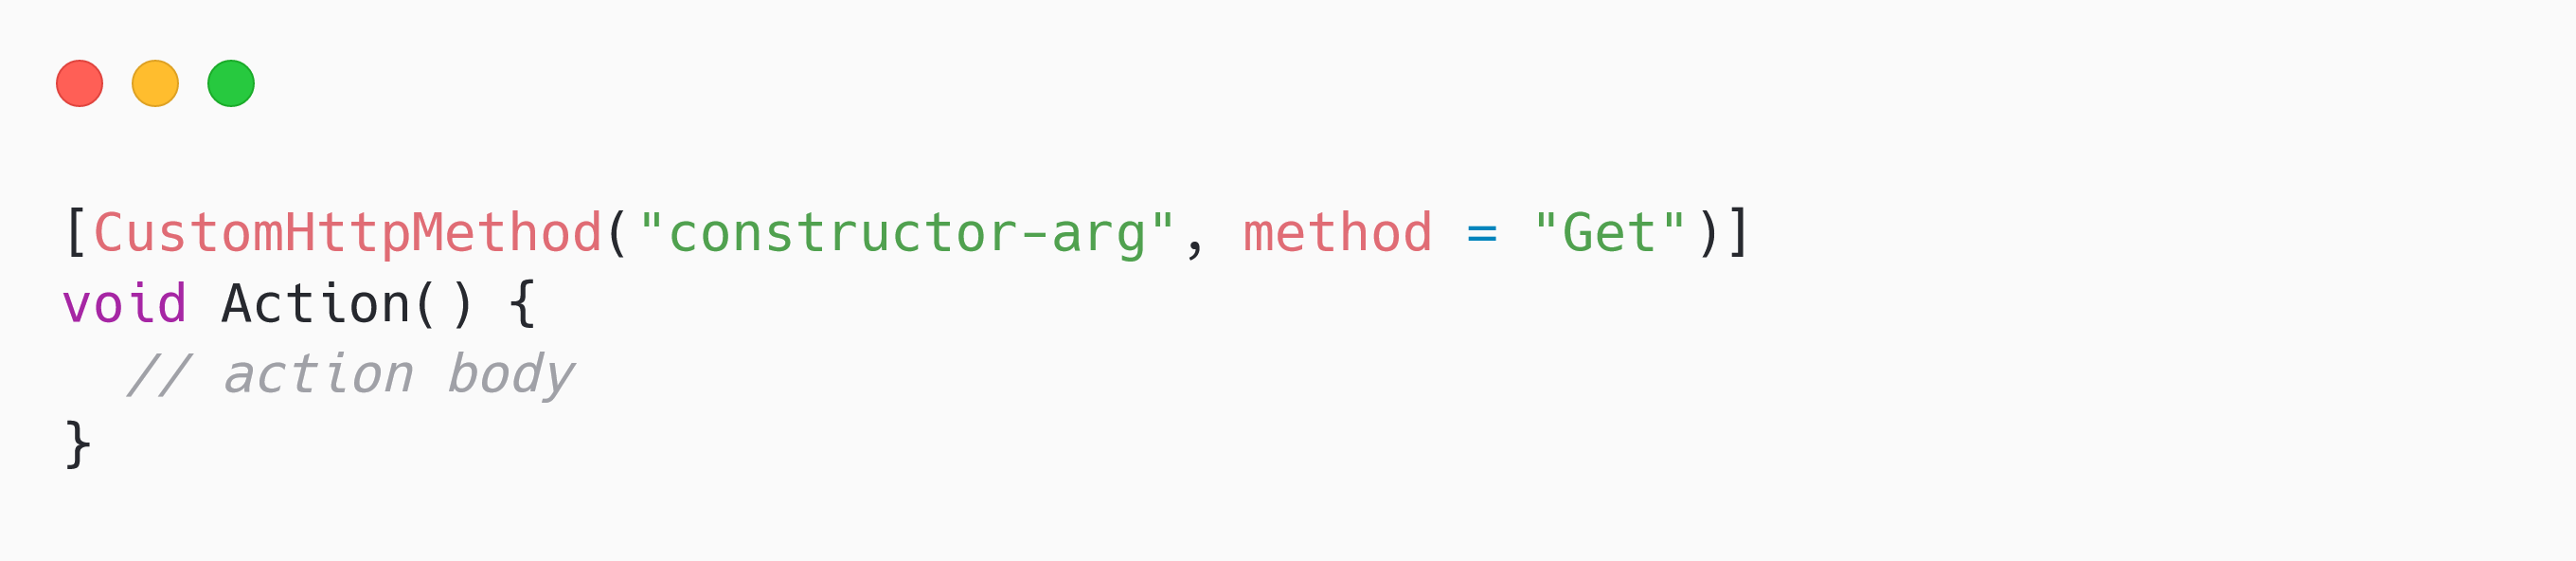
\includegraphics[width=1\textwidth]{graphics/custom-http-method.png}
\caption{An action with a custom \texttt{IActionHttpMethodProvider} attribute}
\label{fig:custom-http-method}
\end{figure}

Figure \ref{fig:custom-http-method} displays a custom attribute that implements the IActionHttpMethodProvider. The attribute holds a constructor argument and a named property. In our case, the named property, "method," declares the HTTP method our action supports. However, the source generator can't determine this, as this is a user-defined IActionHttpMethodProvider attribute. Therefore, to get the correct values, we instantiate the attributes with the same arguments defined in the source code and extract the value of the HttpMethods property, which will contain the correct value at runtime. Attributes in C\# can have both constructor arguments (in our example, shown as \texttt{"constructor-arg"}) and named properties (shown as \texttt{method = "Get"}). However, the syntax for instantiating a new object differs from defining an attribute. For this reason, we must ensure both constructor arguments and named properties are included when creating attributes in the generated source code. Figure \ref{fig:custom-attribute-creation} shows how the attribute in Figure \ref{fig:custom-http-method} has to be instantiated to guarantee the support of the IActionHttpMethodProvider interface.

\begin{figure}[H]
\centering
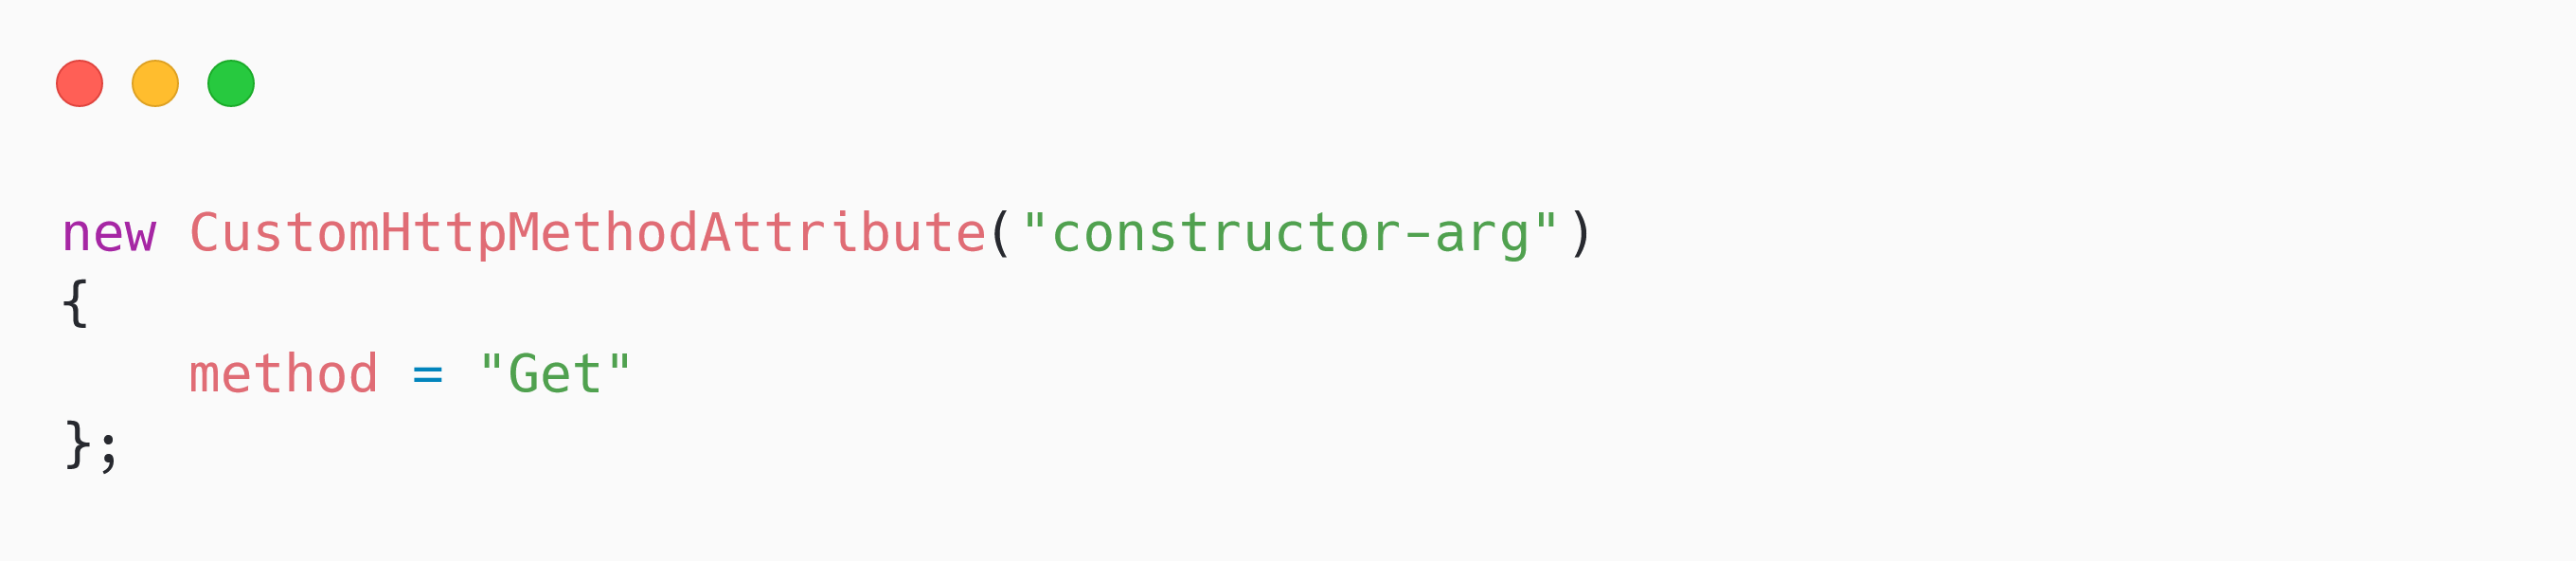
\includegraphics[width=1\textwidth]{graphics/custom-attribute-creation.png}
\caption{Instantiating the \texttt{CustomHttpMethodAttribute} in the generated code}
\label{fig:custom-attribute-creation}
\end{figure}

\subsection{Example output}

This section contains a short example to demonstrate what our source generator creates. We take a small application with a single controller as a starting point. The controller's source code can be seen in Figure \ref{fig:example-controller}.

\begin{figure}[H]
\centering
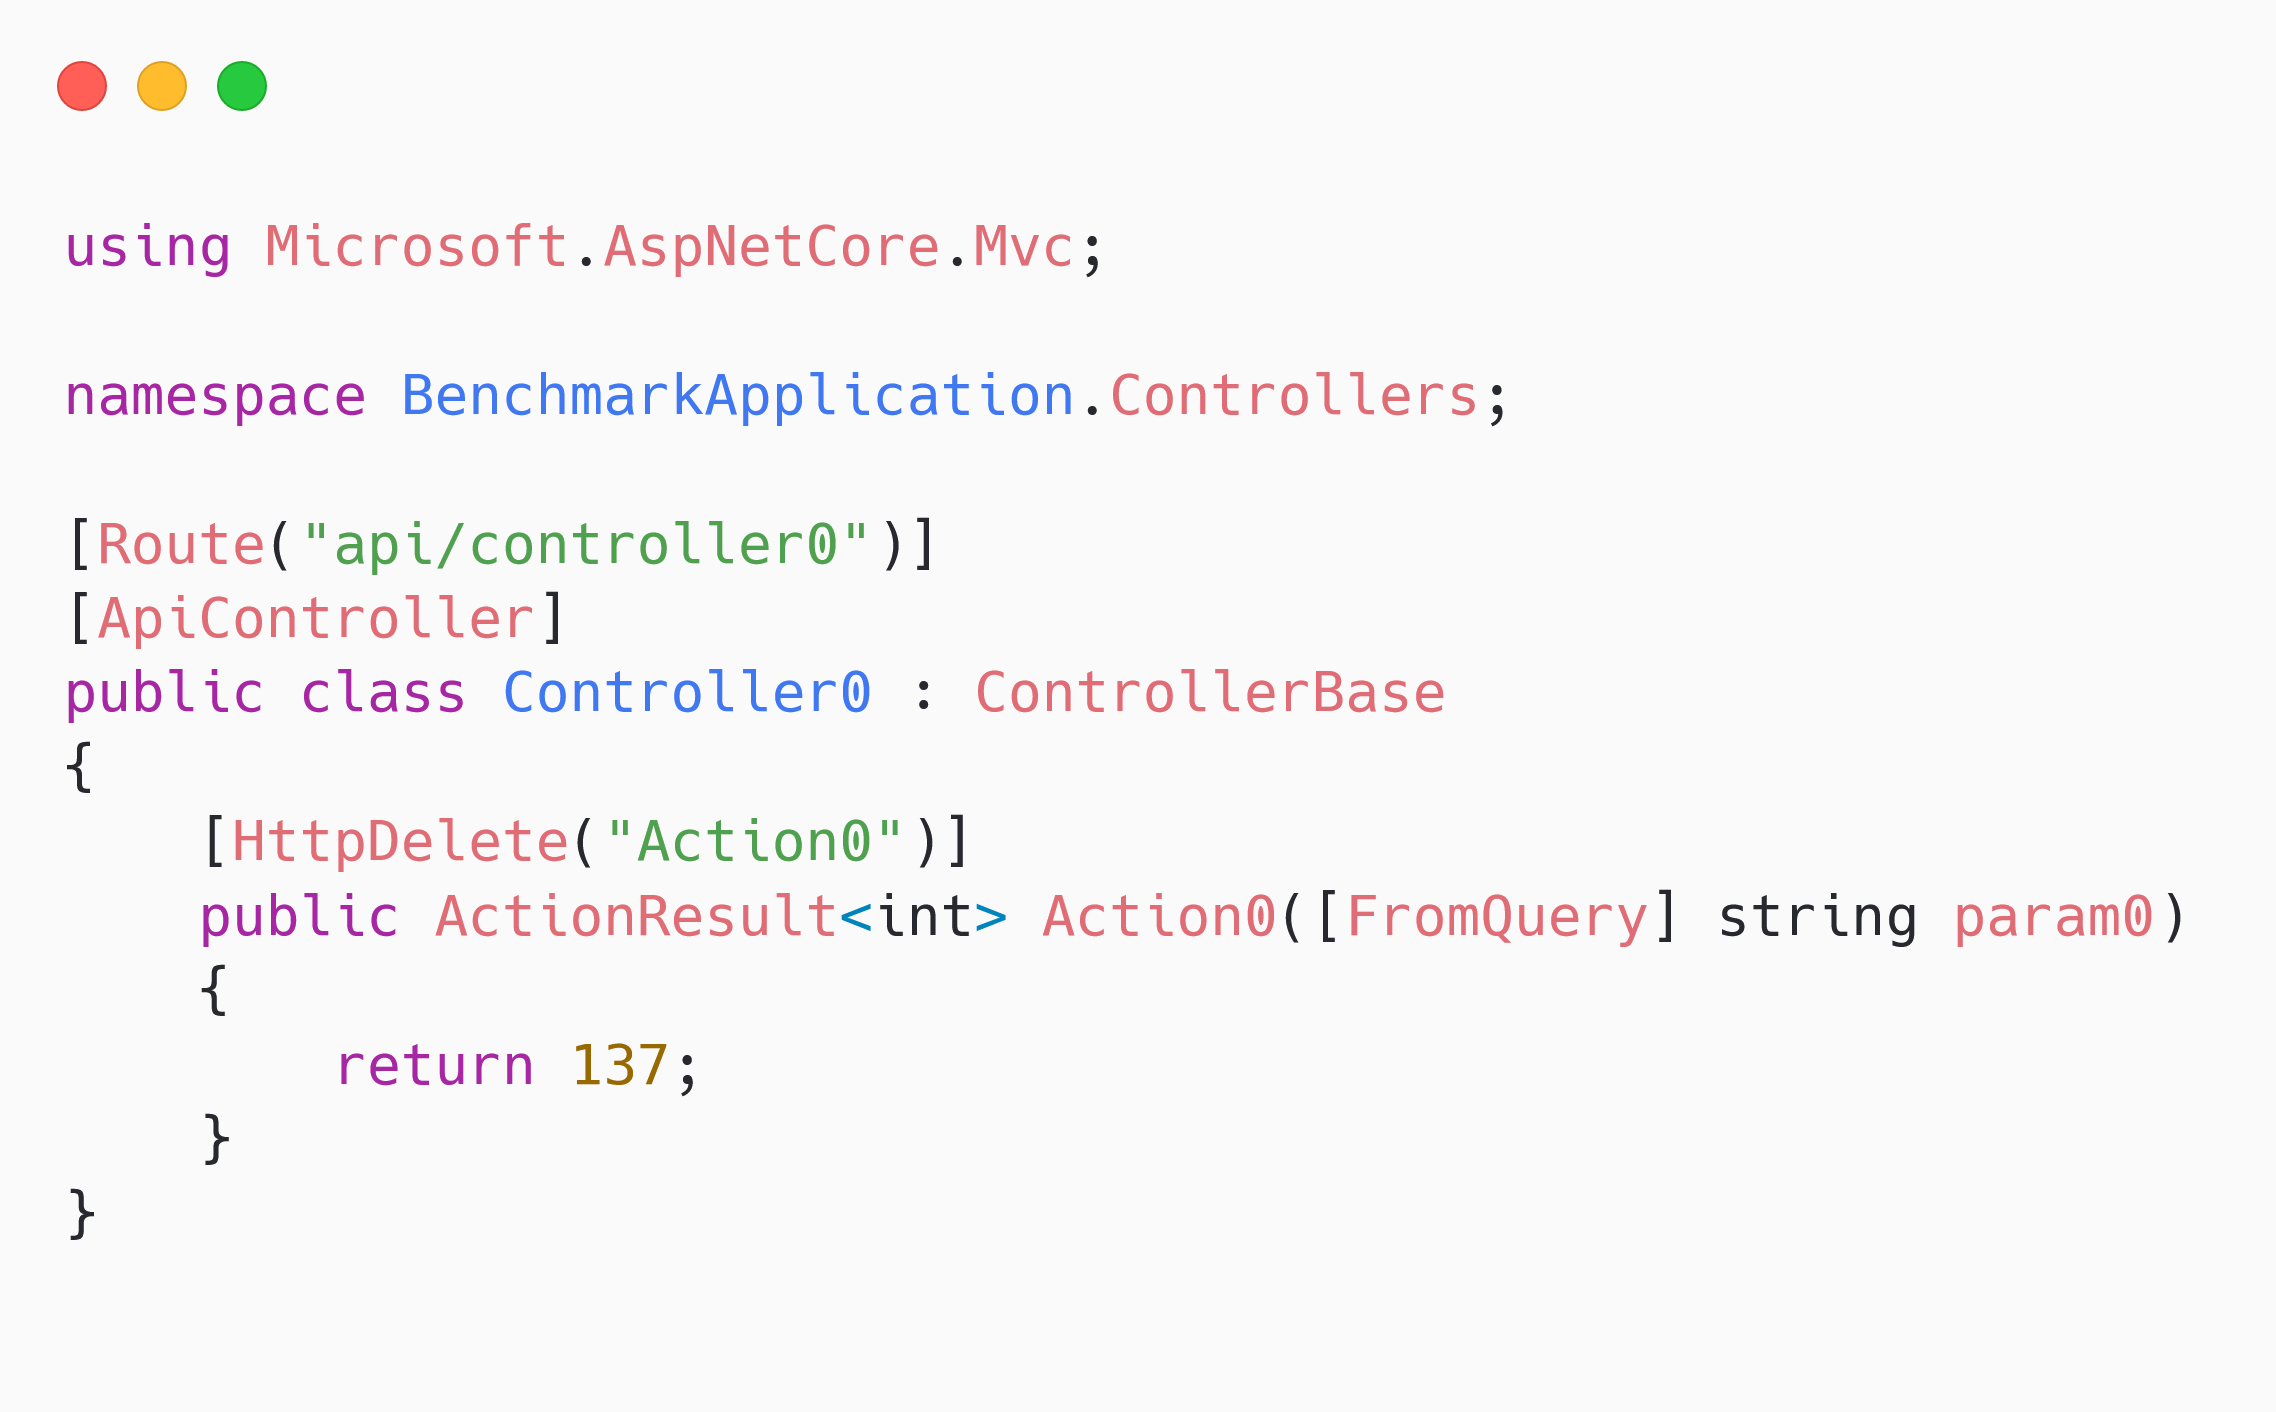
\includegraphics[width=1\textwidth]{graphics/example-controller.png}
\caption{The source code of a trivial controller with an action}
\label{fig:example-controller}
\end{figure}

The controller contains two attributes required by the routing middleware and has a single action. The action will respond only to HTTP requests with the \texttt{Delete} method because of the \texttt{HttpDelete} attribute. The source generator will detect this class and generate an according \texttt{IApplicationModelProvider} class with the content shown in Figure \ref{fig:example-application-model-provider}.

\newgeometry{top=3cm}  % Change the top margin to 3 cm

\begin{figure}[H]
\centering
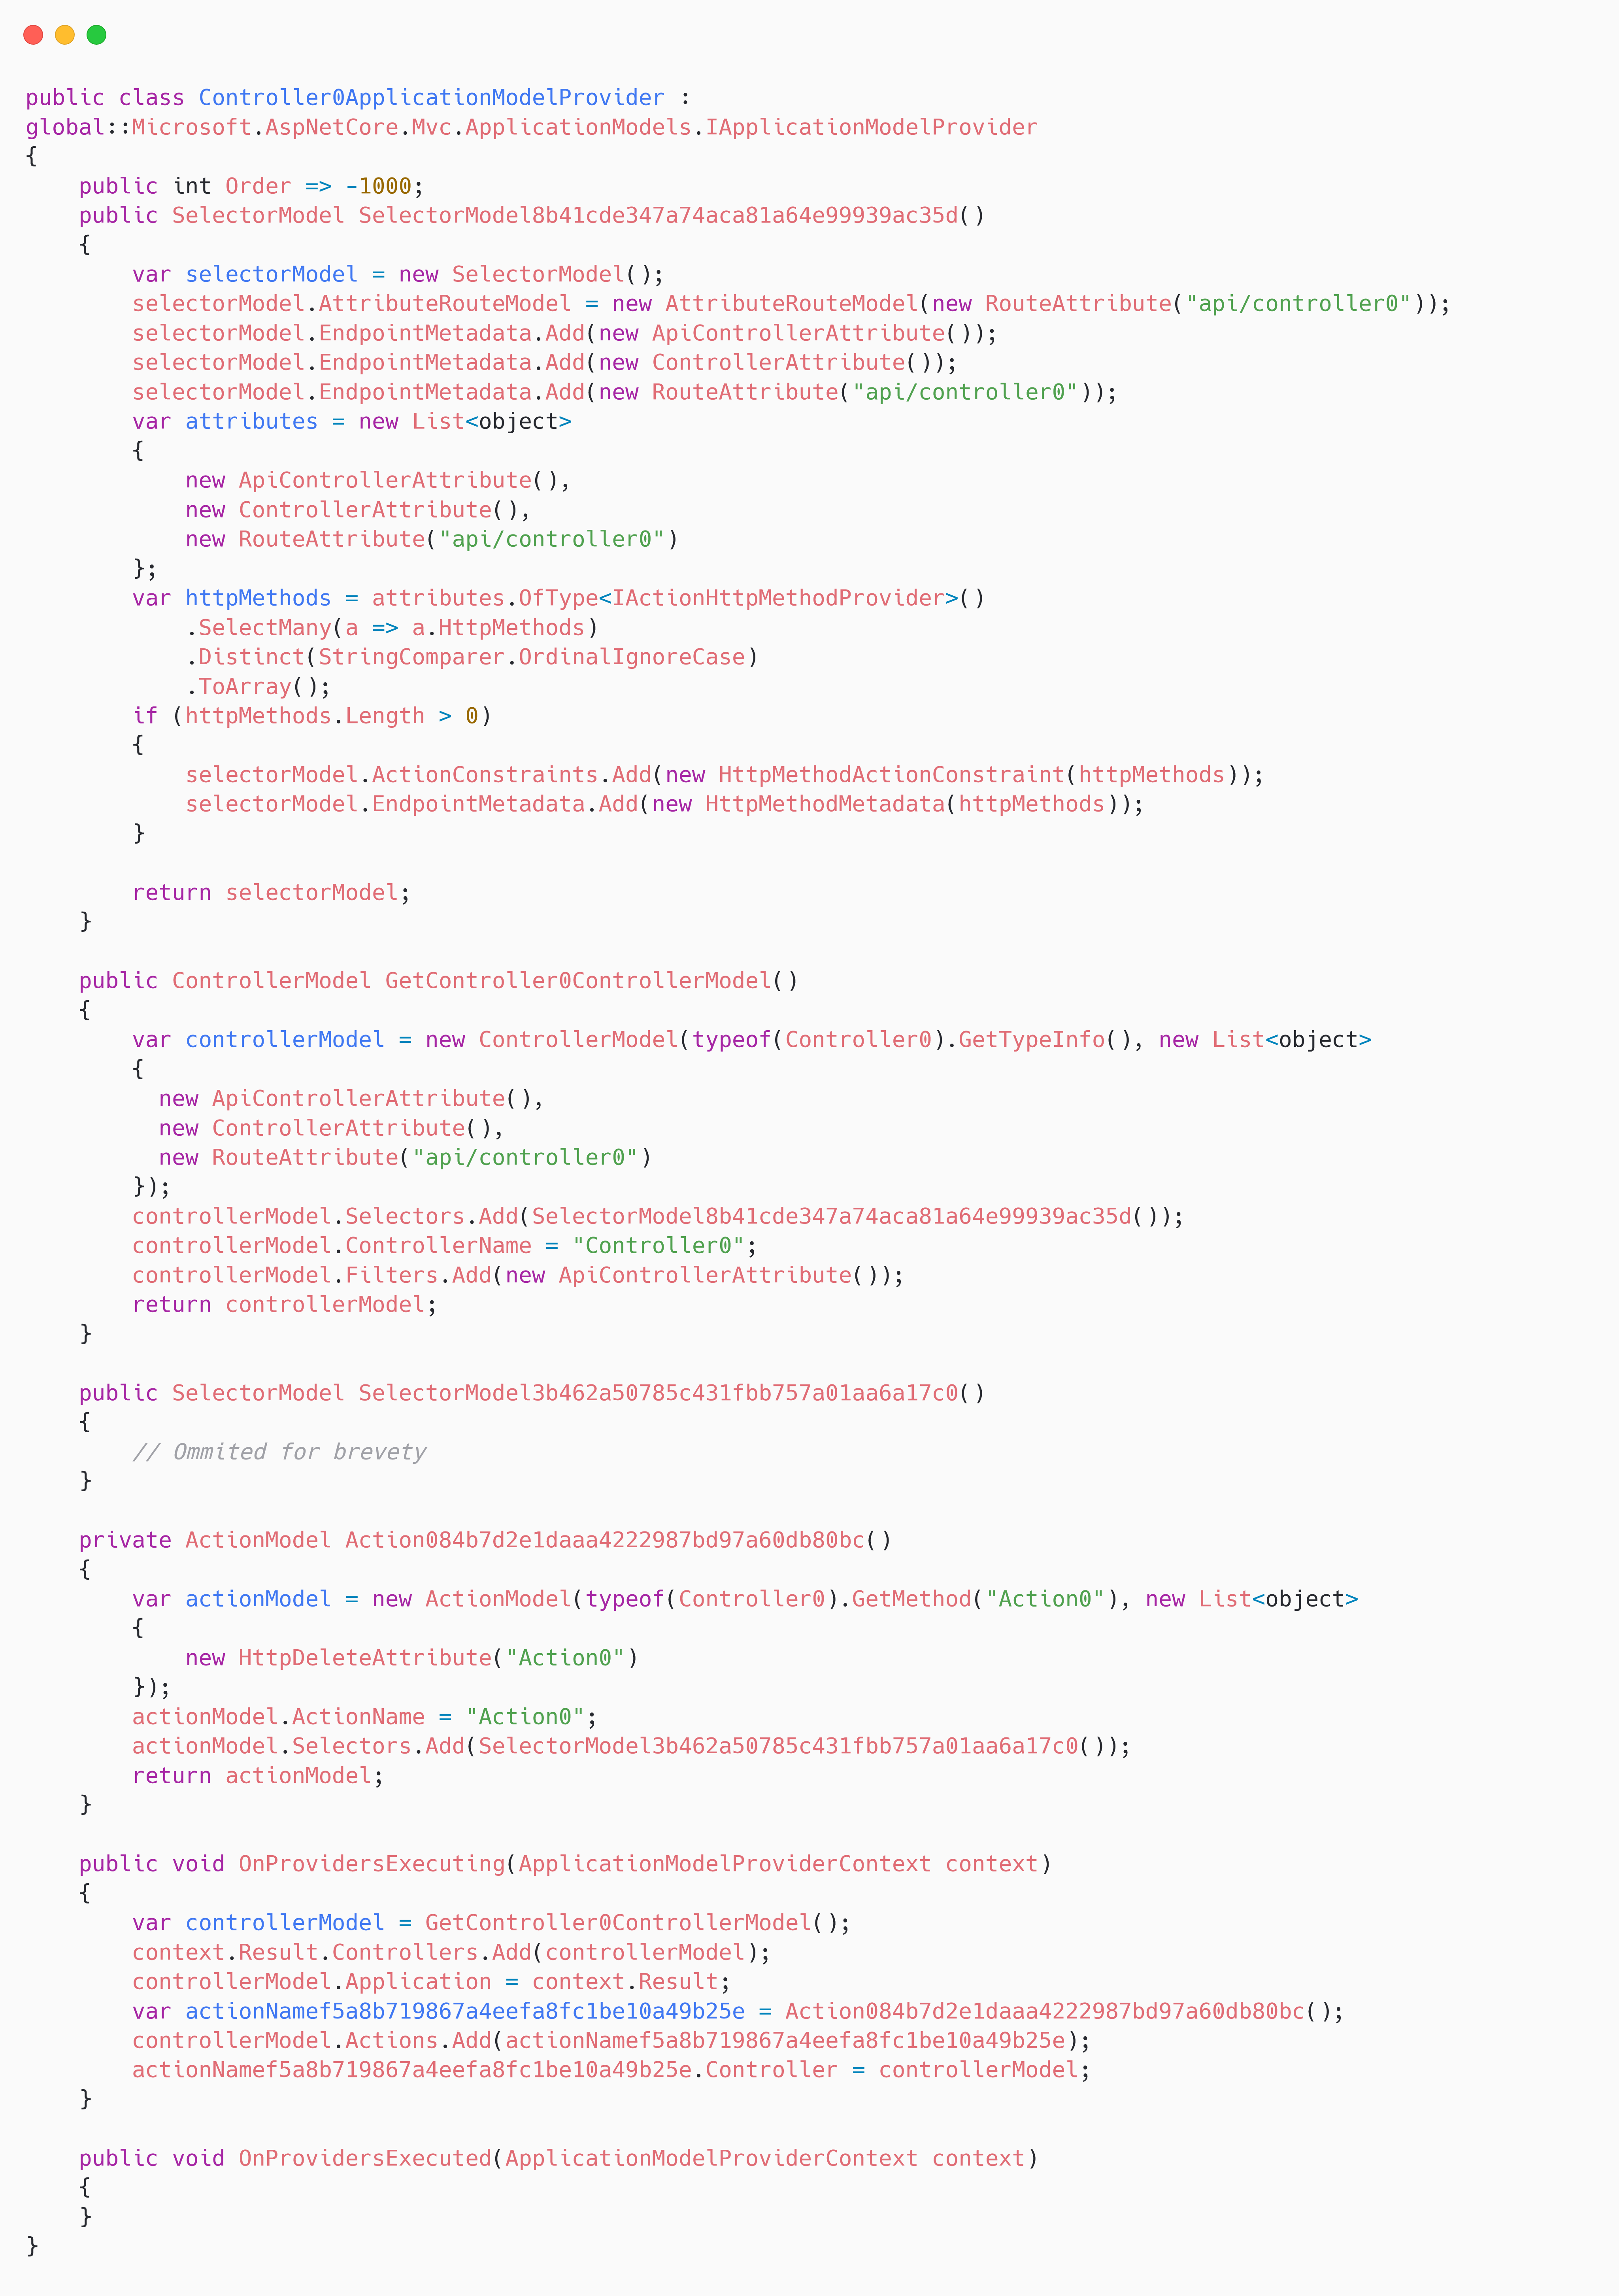
\includegraphics[width=\linewidth]{graphics/example-application-model-provider.png}
\caption{Generated source code for the previously declared trivial controller}
\label{fig:example-application-model-provider}
\end{figure}

\restoregeometry  % Restore the original page layout

The code has been modified for better readability. The generated code uses full name resolution for every, as it is shown on line two for \texttt{IApplicationModelProvider}. Every type is declared beginning with the \texttt{global} namespace followed by the types namespace. This allows us to omit most imports and prevents any naming conflicts. Once such a \texttt{IApplicationModelProvider} class has been generated for each controller, the source generator creates an extension method for the \texttt{IServiceCollection}. It is an extension method to make the usage of the static action discovery as similar as possible to the existing dynamic action discovery. Figure \ref{fig:add-static-mvc} shows an example output for an application with the same single controller as shown in Figure \ref{fig:example-controller}.

\begin{figure}[H]
\centering
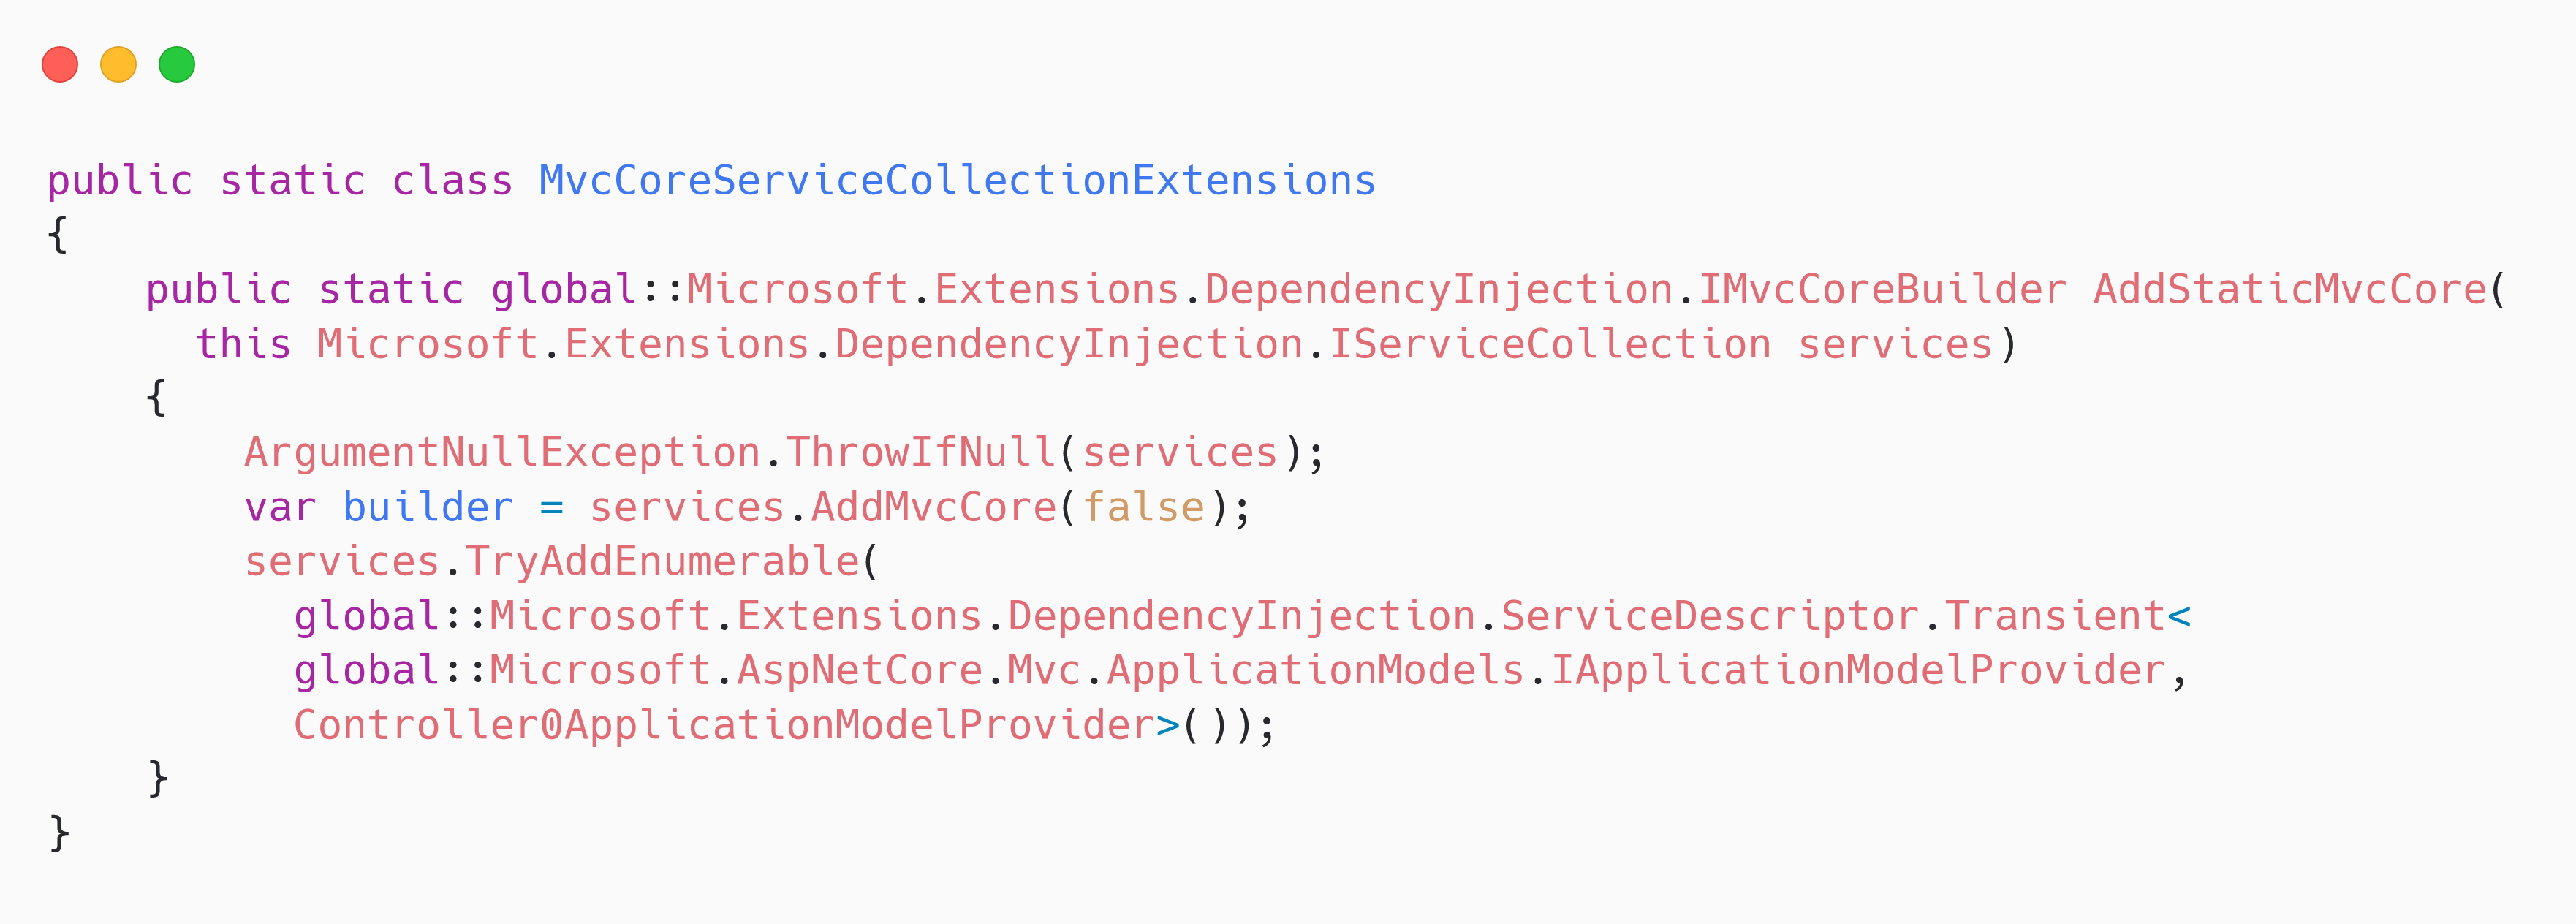
\includegraphics[width=\linewidth]{graphics/add-static-mvc-core.png}
\caption{Generated extension method to add static action discovery for a single controller application}
\label{fig:add-static-mvc}
\end{figure}

As one can see, this method first adds the services required by an MVC application to the builder. The \texttt{false} keyword of the \texttt{AddMvcCore} method omits the dynamic action discovery. It then adds all the generated \texttt{IApplicationModelProvider} to the application's DI container. After this \texttt{AddStaticMvcCore} method is called, the static action discovery has been successfully added and can be executed by running \texttt{MapControllers} after the application is built.

\subsection{Using the source generators in a custom application}

In order to leverage the static action discovery we've created, it's necessary to reference the MVC generators project from ASP.NET Core. This project is not publicly available at the time of writing this thesis, as the required changes have not been merged into Microsoft's official repository and are only accessible through a separate fork. The project will be released once these changes are integrated as part of the official ASP.NET Core package family. Figure \ref{fig:package-reference} illustrates the method for referencing this project within the \texttt{.csproj} file. The \texttt{OutputItemType} needs to be set to \texttt{Analyzer}, which informs the compiler that this project contains source generators to be executed. The \texttt{ReferenceOutputAssembly} should be set to \texttt{false} to ensure the built executable does not package the generator's dynamic link library (DLL).

\begin{figure}[H]
\centering
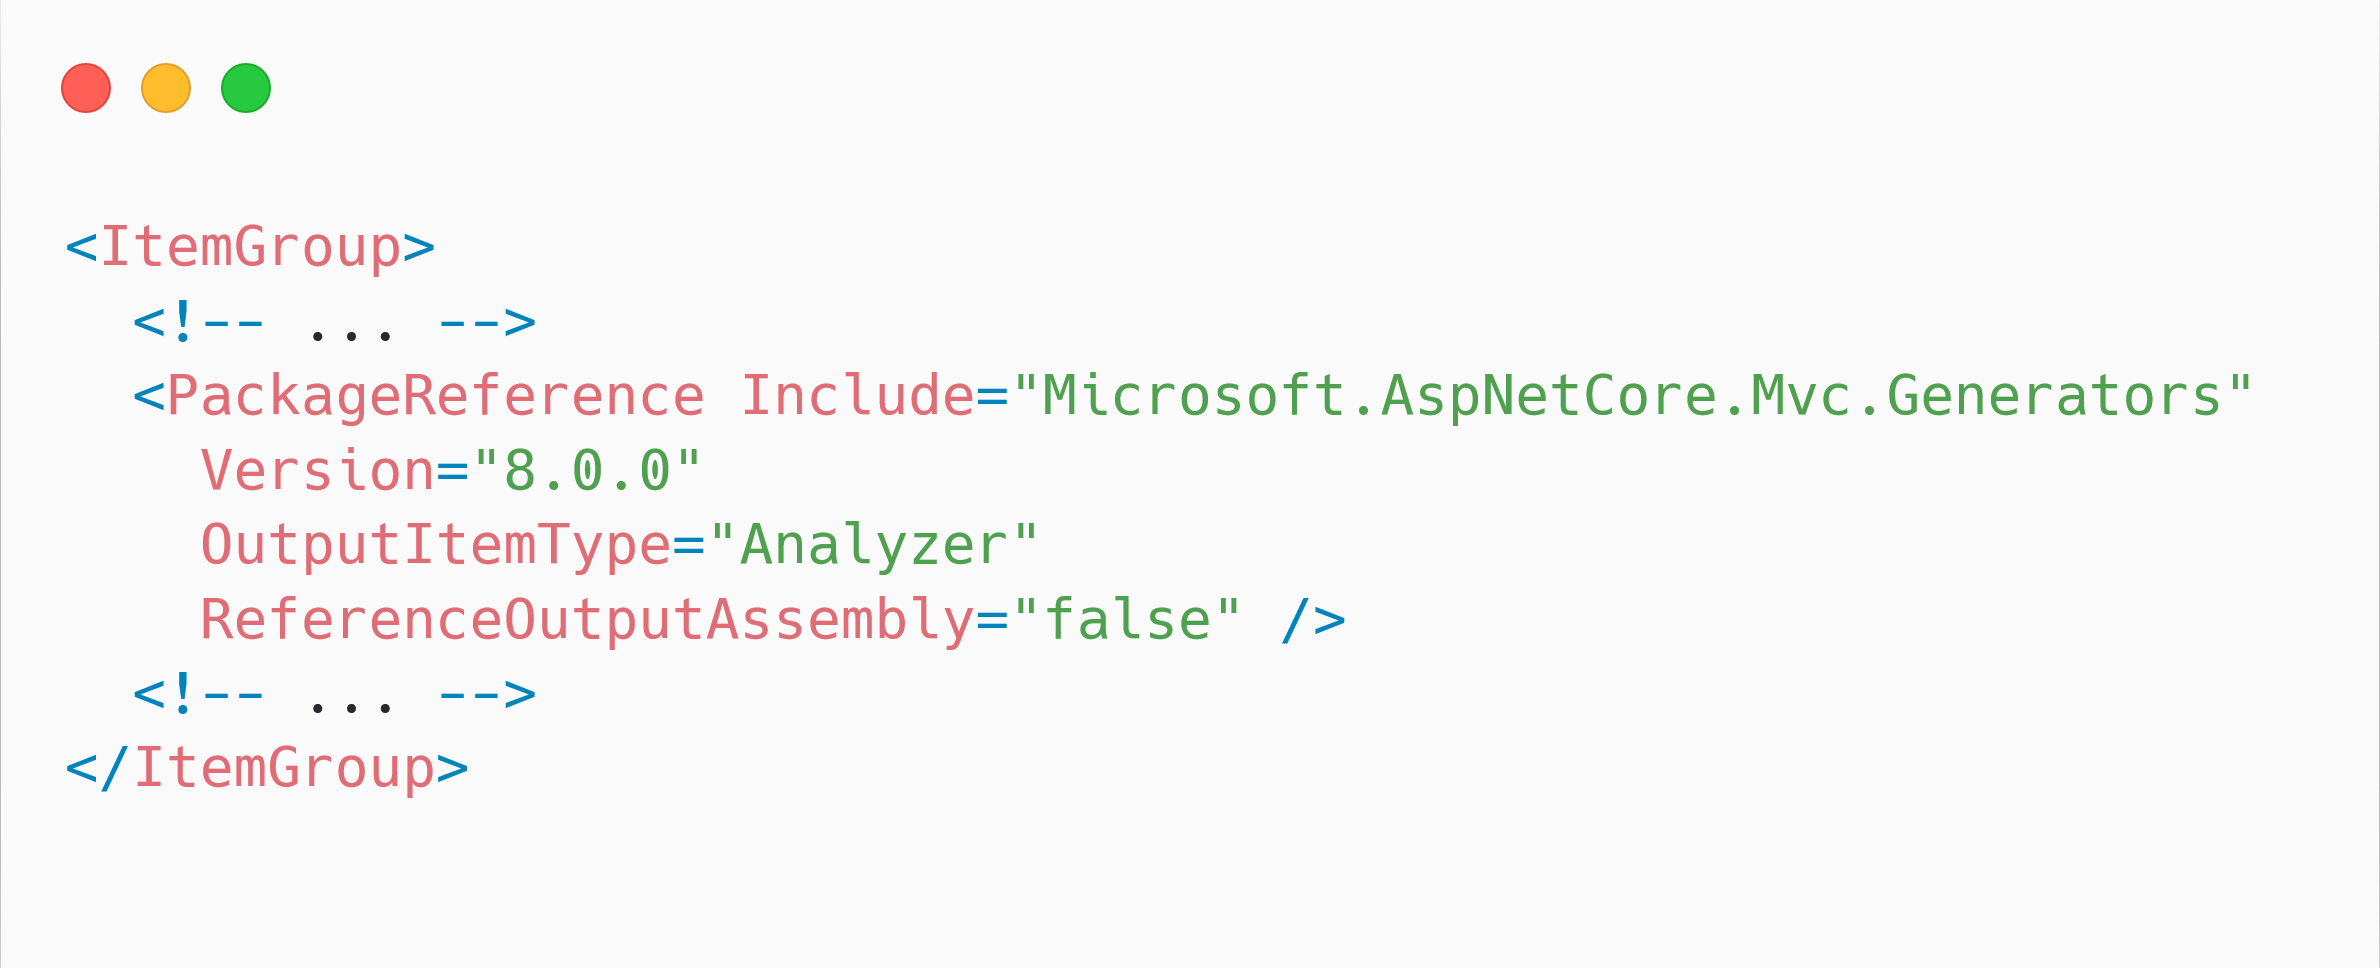
\includegraphics[width=\linewidth]{graphics/package-reference.png}
\caption{Example project file snippet that references the static action discovery source generators}
\label{fig:package-reference}
\end{figure}

Once the generator project is referenced, the compiler will automatically generate the \texttt{AddStaticMvcCore} extension method with the controllers of the target application. Figure \ref{fig:static-startup-method} shows that it can then be used to create a complete application that uses static action discovery.

\begin{figure}[H]
\centering
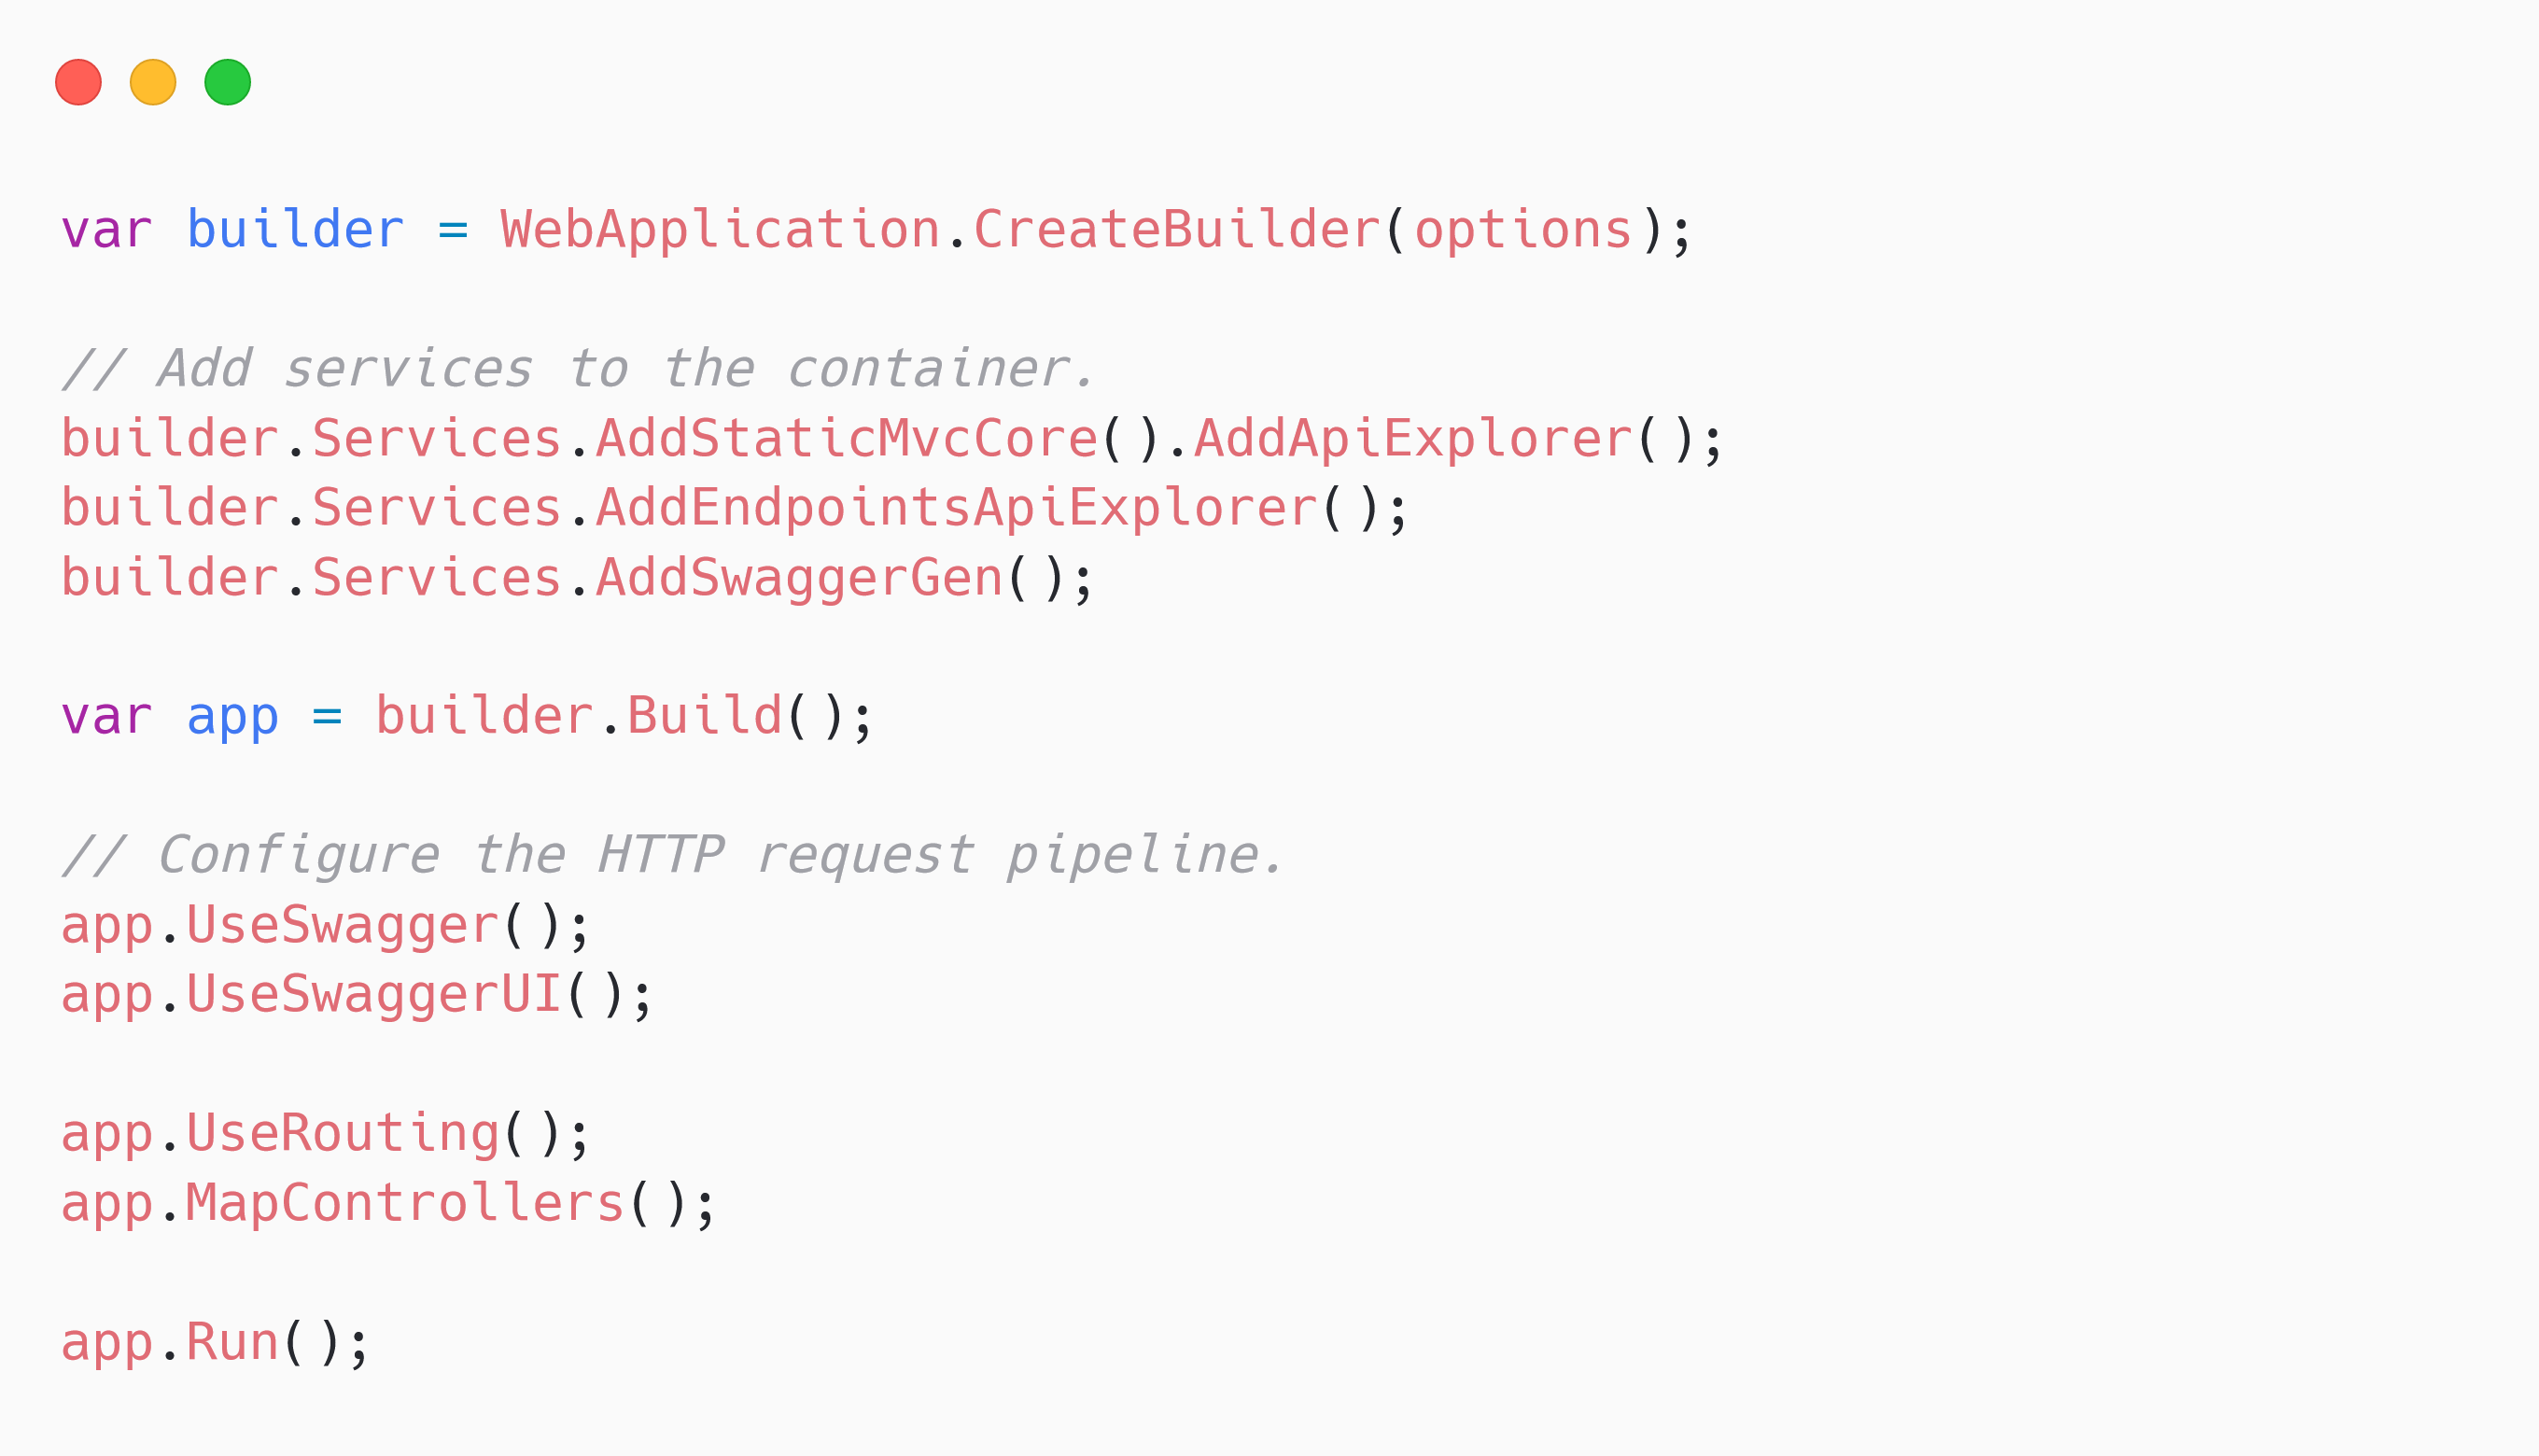
\includegraphics[width=\linewidth]{graphics/startup-method.png}
\caption{Example main setup code for an ASP.NET Core application that uses static action discovery}
\label{fig:static-startup-method}
\end{figure}